\documentclass[12pt]{article}
\usepackage{graphicx}
\usepackage[utf8]{inputenc}
\usepackage{epsfig}
\usepackage{float,graphicx}
\usepackage{listings}
\usepackage{xcolor}
\usepackage{hyperref}
\usepackage{amssymb}
\usepackage{amsmath}
\usepackage{pdfpages}
\usepackage{indentfirst}

\definecolor{codegreen}{rgb}{0,0.6,0}
\definecolor{codegray}{rgb}{0.5,0.5,0.5}
\definecolor{codepurple}{rgb}{0,0,0}
\definecolor{backcolour}{rgb}{1,1,1}

\hypersetup{
 colorlinks,
 citecolor=blue,
 linkcolor=blue,
 urlcolor=blue}

\lstdefinestyle{mystyle}{
    backgroundcolor=\color{backcolour},
    commentstyle=\color{codegreen},
    keywordstyle=\color{black},
    numberstyle=\tiny\color{codegray},
    stringstyle=\color{codepurple},
    basicstyle=\ttfamily\footnotesize,
    breakatwhitespace=false,
    breaklines=true,
    captionpos=b,
    keepspaces=true,
    numbers=left,
    numbersep=5pt,
    showspaces=false,
    showstringspaces=false,
    showtabs=false,
    tabsize=2
}

\lstset{style=mystyle}
\title{\textbf{Reflection of National Culture in Civil Hospital, Jalna}\\
HS490: Course Project}

\author{Yash Paritkar\\
Roll Number: 210070096\\
\\
Instructor: Prof. Pooja Purang}

\date{05 April, 2023}

\begin{document}
\maketitle

\newpage
\section*{Abstract}
\addcontentsline{toc}{section}{Abstract}
This report explores the reflection of national culture on Indian government organizations. The study draws on Hofstede's dimensions of culture to analyze the impact of cultural values on the functioning of Indian government organizations. Specifically, the report examines the dimensions of power distance, individualism vs collectivism, masculinity vs femininity, uncertainty avoidance, and long-term vs short-term orientation.

The findings of the study indicate that Indian government organizations reflect the cultural values of the society they operate in. Power distance is high in Indian culture, and this is reflected in the hierarchical structure of government organizations. Collectivism is also a significant cultural value in India, and this is reflected in the emphasis on teamwork and group decision-making in government organizations.

Masculinity and femininity were found to be relatively balanced in Indian culture, and this is reflected in the diverse roles of men and women in government organizations. Uncertainty avoidance was found to be high in Indian culture, and this is reflected in the preference for established rules and procedures in government organizations. Finally, long-term orientation was found to be a significant cultural value in India, and this is reflected in the emphasis on long-term planning and policy-making in government organizations.


\newpage
\section*{Acknowledgement}
\addcontentsline{toc}{section}{Acknowledgement}
I would like to start by expressing my gratitude to Prof. Pooja Purang for giving me this chance and guiding me while I was writing this report. I also want to thank my father, Dr. Paritkar, for reviewing the survey's questionnaire and assisting me conduct it. I want to express my gratitude to Sailee Biwalkar for helping me with the endeavour. I'd like to express my gratitude to my friend Siddhant Dongare for perfoming peer review of the questionnaire. I would like to thank my friend Veeresh for reviewing the report. Finally, humble thanks to all medical professionals who paarticipated in the survey and provided their valuable time.

\newpage
\tableofcontents
\newpage
\listoffigures
\newpage
\listoftables

\newpage
\section{Introduction to National Culture}
\subsection{What is Culture?}
\begin{quote}
    Culture is collective programming of the mind which distuinguishes the member of one social group from another.\hfill -Greet Hofstede
\end{quote}

Culture refers to the shared beliefs, values, customs, behaviours, and artefacts that characterize a particular group or society. It includes every aspect of society, be it food, music, or religion. The culture can be learned and is passed on from generation by generation.

One common theory is that culture developed as a way for early humans to adapt to their environments and survive in challenging conditions. For example, the development of agriculture and animal domestication allowed early humans to settle in one place and build complex societies, which led to the development of language, art, religion, and other cultural practices. Hence a group of people having the same culture can be identified with how they perceive the environment around them.

Initially, anthropologists believed that culture was a product of biological evolution and that cultural evolution depended exclusively on physical conditions. Today’s anthropologists no longer believe it is this simple. Neither culture nor biology is solely responsible for the other. They interact in very complex ways, which biological anthropologists will be studying for years to come.

The culture us characterized by few basic elements. The elements of culture are
\begin{itemize}
    \item Symbols: anything which carries a particular meaning recognized by people of same culture
    \item Language: system of symbols with which people communicate
    \item Values: culturally-defined standards that serve as broad guidelines
    \item Beliefs: specific statements that people hold to be true
    \item Norms: rules and expectations by which a society guides the behavior of its members
\end{itemize}

Although culture is a very big umbrella term that includes various terms social behaviour, institutions and norms, there have been attempts made to try to analyse the culture. The first attempt in modern times was made by Samuel Pofendorf, \textit{"culture"}, he quoted, \textit{"refers to all the ways in which human beings overcome their original barbarism, and through artifice, become fully human."}

\subsection{National Culture}

National culture refers to the shared beliefs, values, customs, behaviours, and artefacts that characterize a particular country or nation. It is a complex and multifaceted concept that has a significant impact on every aspect of society, including business, education, government, and social interactions. Understanding national culture is vital for individuals and organizations that operate in multiple countries or interact with people from diverse cultural backgrounds.

National culture is affected by wide ranging factors such as :
\begin{itemize}
    \item History
    \item Geography
    \item Religion
    \item Language
    \item Political systems
\end{itemize}

As is common knowledge, every country has a unique history. Different countries' histories are unique; some were highly wealthy, some had limited resources, some frequently experienced natural disasters, and some had fertile territory. The morals and emblems of various nations vary. Different nations have various forms of administration. These variables, which are particular to each country, resulting in those nations having distinctive cultures.

\subsection{Hofstede's Study on National Culture}

The first significant attempt at analysing the culture of people according to their nationalities was made by Geert Hofstede. This was carried out in the 1970s. It was significant research for understanding national culture. Many multinational corporations, who were attempting to expand into new nations as globalisation grew throughout the globe, saw the importance of this study.

Hofstede's cultural dimensions theory is a framework for cross-cultural communication developed by Geert Hofstede. It shows the effects of a society's culture on the values of its members and how these values relate to behaviour, using a structure derived from factor analysis. In 1965, Hofstede founded the personnel research department of IBM Europe (which he managed until 1971). Between 1967 and 1973, he executed a large survey study regarding differences in national values across the worldwide subsidiaries of this multinational corporation: he compared the answers of 117,000 IBM-matched employee samples on the same attitude survey in different countries. He first focused his research on the 40 largest countries and then extended it to 50 countries and three regions, \textit{"at that time probably the largest matched-sample cross-national database available anywhere."} The theory was one of the first quantifiable theories that could be used to explain the observed differences between cultures.

Initially he proposed four dimensions along which cultural values could be analyzed: 
\begin{itemize}
    \item individualism-collectivism: degree to which people in a society are integrated into groups
    \item uncertainity avoidance: a society's tolerance to ambiguity
    \item power distance (strength of social hierarchy): the extent to which the less powerful members of organizations and institutions (like the family) accept and expect that power is distributed unequally
    \item masculinity-femininity (task-orientation versus person-orientation): masculinity is defined as "a preference in society for achievement, heroism, assertiveness, and material rewards for success"
\end{itemize}
Later on, two extra dimensions were added to the list. The fifth one was added by independent researchers in Hong-Kong, long-term orientation and the last one was added recently in 2010 by Hofstede, indulgence versus self-restraint.

\section{National Culture of India}

\subsection{Introduction}

India's national culture is distinctive. India has been thriving since primordial times. Because of its size, the widespread practice of faith, the availability of food due to its fertile land, and the wide range of climates and landforms throughout the nation, there is a very diverse population. Politically and demographically, this nation was formed as a result of the people's fight against repeated foreign invasions over thousands of years and 250 years of slavery as a colony of an external power 7,000 kilometres away. These all have led to its unique characteristics in national culture.

\subsection{Hofstedes Research on National Culture of India}

Hofstede's research on the national culture of India\cite{ref:Hofstede's research on the national culture of India} has shed light on the complex and diverse cultural landscape of this vibrant nation. By identifying dimensions such as power distance, individualism vs. collectivism, masculinity vs. femininity, uncertainty avoidance, and long-term vs. short-term orientation, Hofstede has provided a framework for understanding the cultural norms and values that shape Indian society.

The result of his cultural analysis can be summarised in Table \ref{Table 1}. We will cover what each individual scores mean in this table.

\begin{table}
    \begin{center}
    \begin{tabular}{|c|c|c|}
        \hline
        Index & India & World Average \\
        \hline
        Power Distance & 77 & 56.5 \\
        Long-Term Orientation & 61 & 48 \\
        Masculinity & 56 & 51 \\
        Individualism & 48 & 40 \\
        Uncertainity Avoidance & 40 & 65 \\
        \hline
    \end{tabular}
    \caption{Cultural dimensions scores for India}
    \label{Table 1}
    \end{center}
\end{table}

\subsubsection{Power Distance}

The power distance measures the extent to which the people with less power are ready to accept unequal power distribution. A high number indicates that the respondents have no trouble following orders from those in higher positions in the hierarchy.

The score of India on this parameter is very high. This indicates that people appreciate vertical hierarchy, and acceptance of un-equal rights is high. This results in accessibility in immediate seniority but not so for the above layer, and loyalty is rewarded for the employee. The power structure tends to be centralized.

\subsubsection{Long-Term Orientation}

This dimension describes how society sees the past and how much it thinks the future will be affected by current actions. Normative societies, which rank poorly on this metric, favour upholding time-honoured customs and standards while being wary of societal change. On the other hand, high-scoring cultures adopt a more practical approach: they promote thrift and efforts in contemporary education as a means of future preparation.

The score of India in this parameter is not tilted significantly to any side. Hence there is no dominant preference among Indians, implying different behaviour for different situations. Nevertheless Indians value thrift and perseverance, they have a high amount of respect for tradition, and they do tend to manipulate things for immediate success.

\subsubsection{Masculinity}

A low score implies that society has feminine characteristics. Hofstede found that in the majority of societies, the characteristics of caring and nurturing are associated with women.

With a score of 56, India can be considered a masculine society. He also found that, overall, India is not equally masculine in all characteristics. In terms of visual display of success and power, Indians are highly masculine, but in daily life, they also show high humility and abstinence with their religious ancient culture.

\subsubsection{Individualism}
A high sense of individualism means inter-personal bonding of people is quite loose, and people tend to think about themselves and their immediate families. In the opposite spectrum, in cultures with high collectivism, members in a group can look at other members for unquestioned loyalty.

Again, the score of India is very balanced and not tilted towards any side. This again shows the selectivity of the Indians towards a few types of groupings. Nevertheless Indians generally associate themselves with certain groups and assign a high status to those in the group and who leave groups feel intense emptiness. Yet religious learning of Indians keep them self-oriented with their concept of death and rebirth.

\subsubsection{Uncertainity Aviodance}

The future can never be known, but you can make yourself prepared for possible futures. This dimension of cultural analysis tests how much people are willing to tolerate uncertain in future.

Compared to the other world, India has a very low score. India is traditionally a patient country where tolerance for the unexpected is high, even welcomed as a break from monotony. People generally do not feel driven and compelled to take action initiatives and comfortably settle into established roles and routines without questioning.

\section{Assesment of Reflecion of National Culture of India in Government Hospital}

Now that we are up to speed on the theory of the national culture of India, we will attempt to evaluate India's national culture in relation to the aforementioned dimension proposed by Hofstede and determine whether we can see the national culture affecting the working of a critical public healthcare offering.

\subsection{Why survey a Government Hospital for Reflection National Culture?}

Surveying a government hospital can be a helpful way to reflect on the national culture of a country for several reasons. Firstly, government hospitals are a crucial part of the healthcare system in most countries, and they provide healthcare services to a large section of the population, including the vulnerable and marginalized sections.

By studying the culture of a government hospital, we can gain insights into the values, norms, and beliefs that shape the healthcare system and its interaction with society. As the name suggests, the government hospitals are managed by the government, and hence they have to follow government regulations and policies\cite{ref: IPCH}. The hospital also offers a unique blend of employees, from well-trained and educated doctors to a sweeper who is 10th pass, offering a wide range of perspectives.

\subsection{Need for Survey}

In order to assess any information, a proper survey needs to be done. Surveys are a valuable tool for collecting data and measuring cultural values and practices. By analysing patterns and trends in the data collected by the survey, one can reach good conclusions which form the basis of any study.

\subsection{Choosing the Sample Set}

While choosing a target audience for the study, we need to have a sample size of good number and quality. In order to study the reflection of national culture in the hospital, which typically has a working staff of about 80 employees, we need to interview about 20. Also, in any given organisation, the role of the employee and his/her vertical position in the hierarchy can affect the answers. Hence we should have people from multiple categories. After considering the accessibility to conduct a survey, the District Government Hospital, Jalna, Maharashtra- 431213, was selected.

\subsection{Creating a Questionnaire}

A good questionnaire is essential for collecting accurate and relevant data in any research project. A well-designed questionnaire helps to ensure that the information collected is reliable, valid, and free from bias.

The importance of a good questionnaire cannot be overstated, as it is the primary tool for collecting data in many research projects. Without a well-designed questionnaire, the data collected may be inaccurate or incomplete, leading to flawed conclusions and recommendations.

The questionnaire used in this assessment was made by studying the book on Organisational Behaviour by Robbins and reading various websites containing national cultures. And it was reviewed by persons from positions to provide multiple perspectives.

\subsection{Analysing the Survey}

Analyzing the survey is an important step in any research project, as it helps to identify patterns and trends in the data collected. The first step in analyzing the survey is to clean and organize the data, removing any errors or inconsistencies that may have arisen during data collection. This was done with utmost care with the help of modern software such as Microsoft Excel and using various graphs and charts.

\section{The Survey}

Using a Google(TM) Form, the project's survey was conducted. Every employee was urged to take part in the survey. In total, 19 responses were given. It was attempted to keep the form from being too lengthy while maintaining the crucial questions in light of the importance of the time of the employees.

\subsection*{Composition of Questionnaire}

The questionnaire consisted of 8 sections, with the first section just being just about writing your name and your role in the organisation. The sections were made according to the dimension of the culture they were trying to enquire about. The eight sections are as following:

\begin{enumerate}
    \item Introduction
    \item Display of emotions
    \item Meetings
    \item Pattern of context
    \item Achievement or Ascription based
    \item Long-Term Orientation
    \item Individualistic or Collectivistic
    \item Control vs Subjugation
\end{enumerate}

The questions were of different types, some being simple factual agree-disagree questions, some multiple choice types and some true-false types. In many questions, the option of the custom answer was kept available as the given options may not be there. Finally, after each section, an optional question to add any comment was incorporated to make sure to collect any specific input any employee might want to give. The questionnaire of the survey can be found in this link \cite{ref: Survey Form}.

\section{Analysis of the Survey}

The initial analysis of the survey was done section-wise the questionnaire in order to simplify the process. After completing the section-wise analysis, the results were combined to analyse the survey as a whole on the five dimensions of the Hofstedes cultural analysis. The full responses of the form can be seen here \cite{ref:Survey Results}.

\subsection{Introduction}

Other than noting the role of the responder, this section doesn't feature any questions, although this can be useful in relating the other answers of the responder. Answers given to this question establish the variety in the responders of the form as the people doing the following roles are there, see Table \ref{responder}

\begin{table}[H]
    \begin{center}
        \begin{tabular}{|c|c|}
            \hline
            Role & Frequency\\
            \hline
            Sister incharge & 1\\
            Medical Officer & 4\\
            Nurse & 4\\
            Opthalmic Officer & 6\\
            Psychiatrist & 1\\
            Skin Specialist & 1\\
            Ward Servent & 1\\
            \hline
        \end{tabular}
        \caption{Role in the organisation}
        \label{responder}
    \end{center}
\end{table}

\subsection{Display of Emotions}

The objective of this section was to test how freely the people can express themselves. This section generated some interesting results. The results can be seen in the Figure \ref{Emotion}.

Although everyone agrees about being able to express emotion in the employee circle, only half of them agree about being tolerant of the others when they express their feelings. As we can expect from a professional, they try to hide their mood while speaking to patients and others. This implies an intermediate amount of both masculinity and individualism.

\begin{figure}
    \centering
    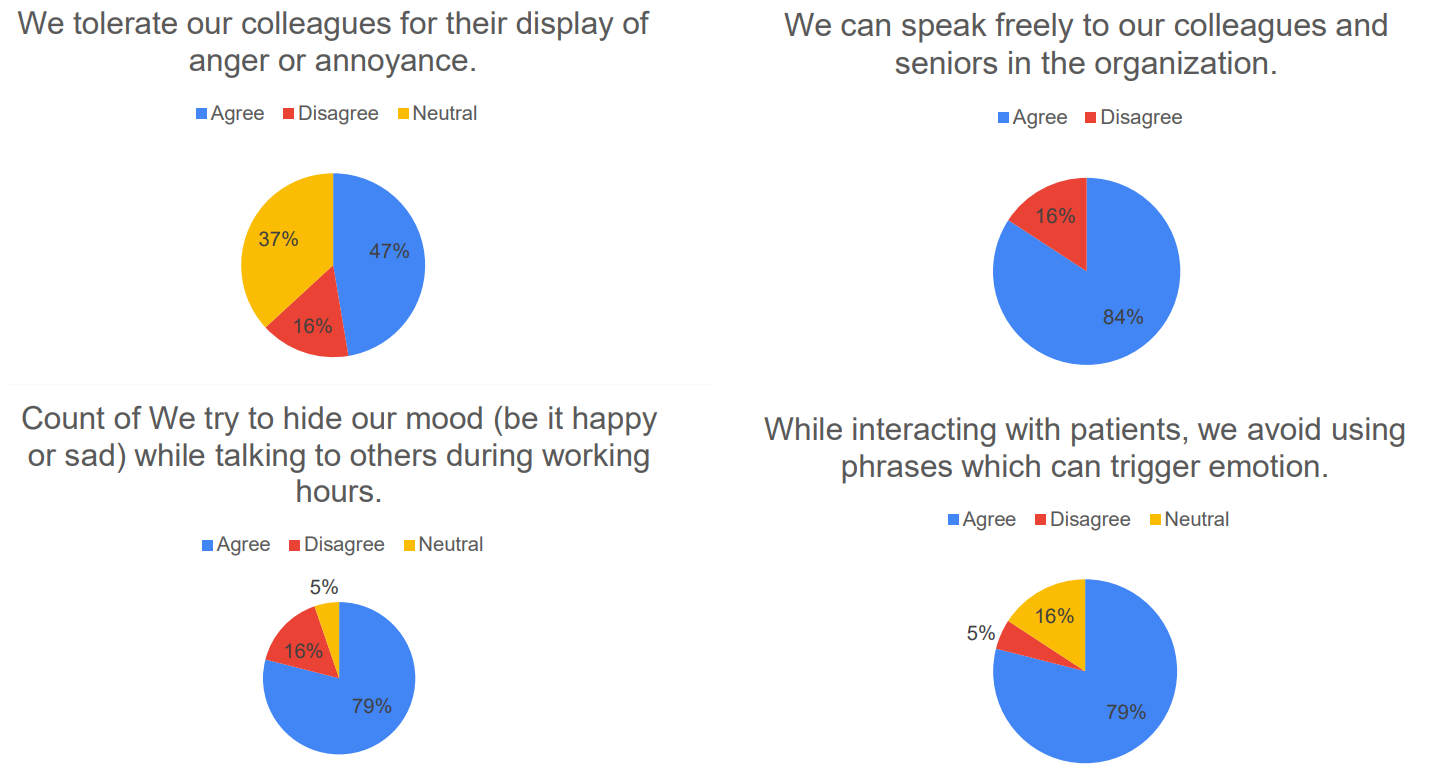
\includegraphics[width = 4.5 in]{Emotion.png}
    \caption{Result of questions on emotion}
    \label{Emotion}
\end{figure}

\subsection{Meetings}

This section try to cover official handling of the organisation specially regarding the procedure of the meeting specially the orientation of time and uncertainity avoidance. In this section four questions were asked. The result of which can be seen in the Figure \ref{meeting}.

\begin{figure}
    \begin{center}
        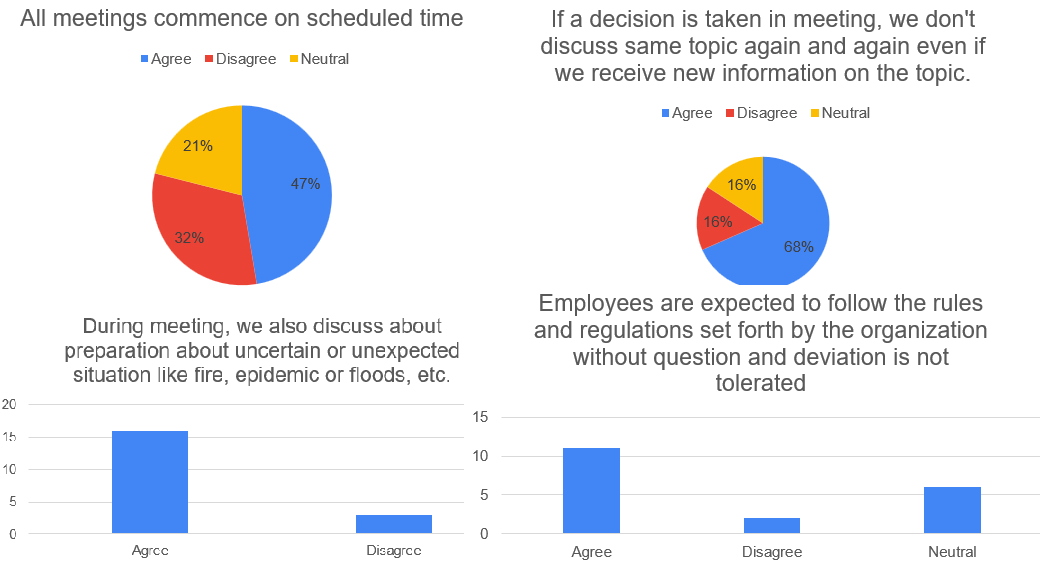
\includegraphics[width = 4in]{Meeting.png}
    \end{center}
    \caption{Responses of Questions based on meeting}
    \label{meeting}
\end{figure}

Just like in typical poly synchronous culture, the meetings tend to get delayed, but the fact that most employees agree that the same topic is not repeated again and again denies total poly synchronism. Also, unlike the typical view of India, the hospital is indeed seen as well prepared against uncertainty which stands out in relation to the general public sector unit.

\subsection{Pattern of context}

A single question was asked on this parameter. This question has a clear majority. Among all the factors which affect the course of action, the position of senior is the one which affects the most. The responses had a about half (~ 52\%) the votes. This strengthens the Hofstedes claim on high power distance.

\subsection{Achievement or Ascription based}

This section tests how the employees are rewarded for their good work. Since most of the employees responded that the employees are not rewarded, this is not very useful to analyse.

An interesting fact is that another question asking for criteria for judging the performance of the employees is again divided into equal halves. Half of the responders agree that actual performance is the metric of their judgement, and half believe that position and people in association make a more significant impact.

\subsection{Long-Term Orientation}

These questions try to ask how the goals of the organisation are with respect to time; they are short-term or long-term. Responses can be seen in Figure \ref{Time}. Now, for the first two questions, both have a narrow majority as stability and procedures. This symbolises the fact that the hospital is looking for long-term goals. Even while this is true, 90\% of the participants agreed that the hospital is pretty fast to incorporating new technology in the medical field.

\begin{figure}
    \begin{center}
        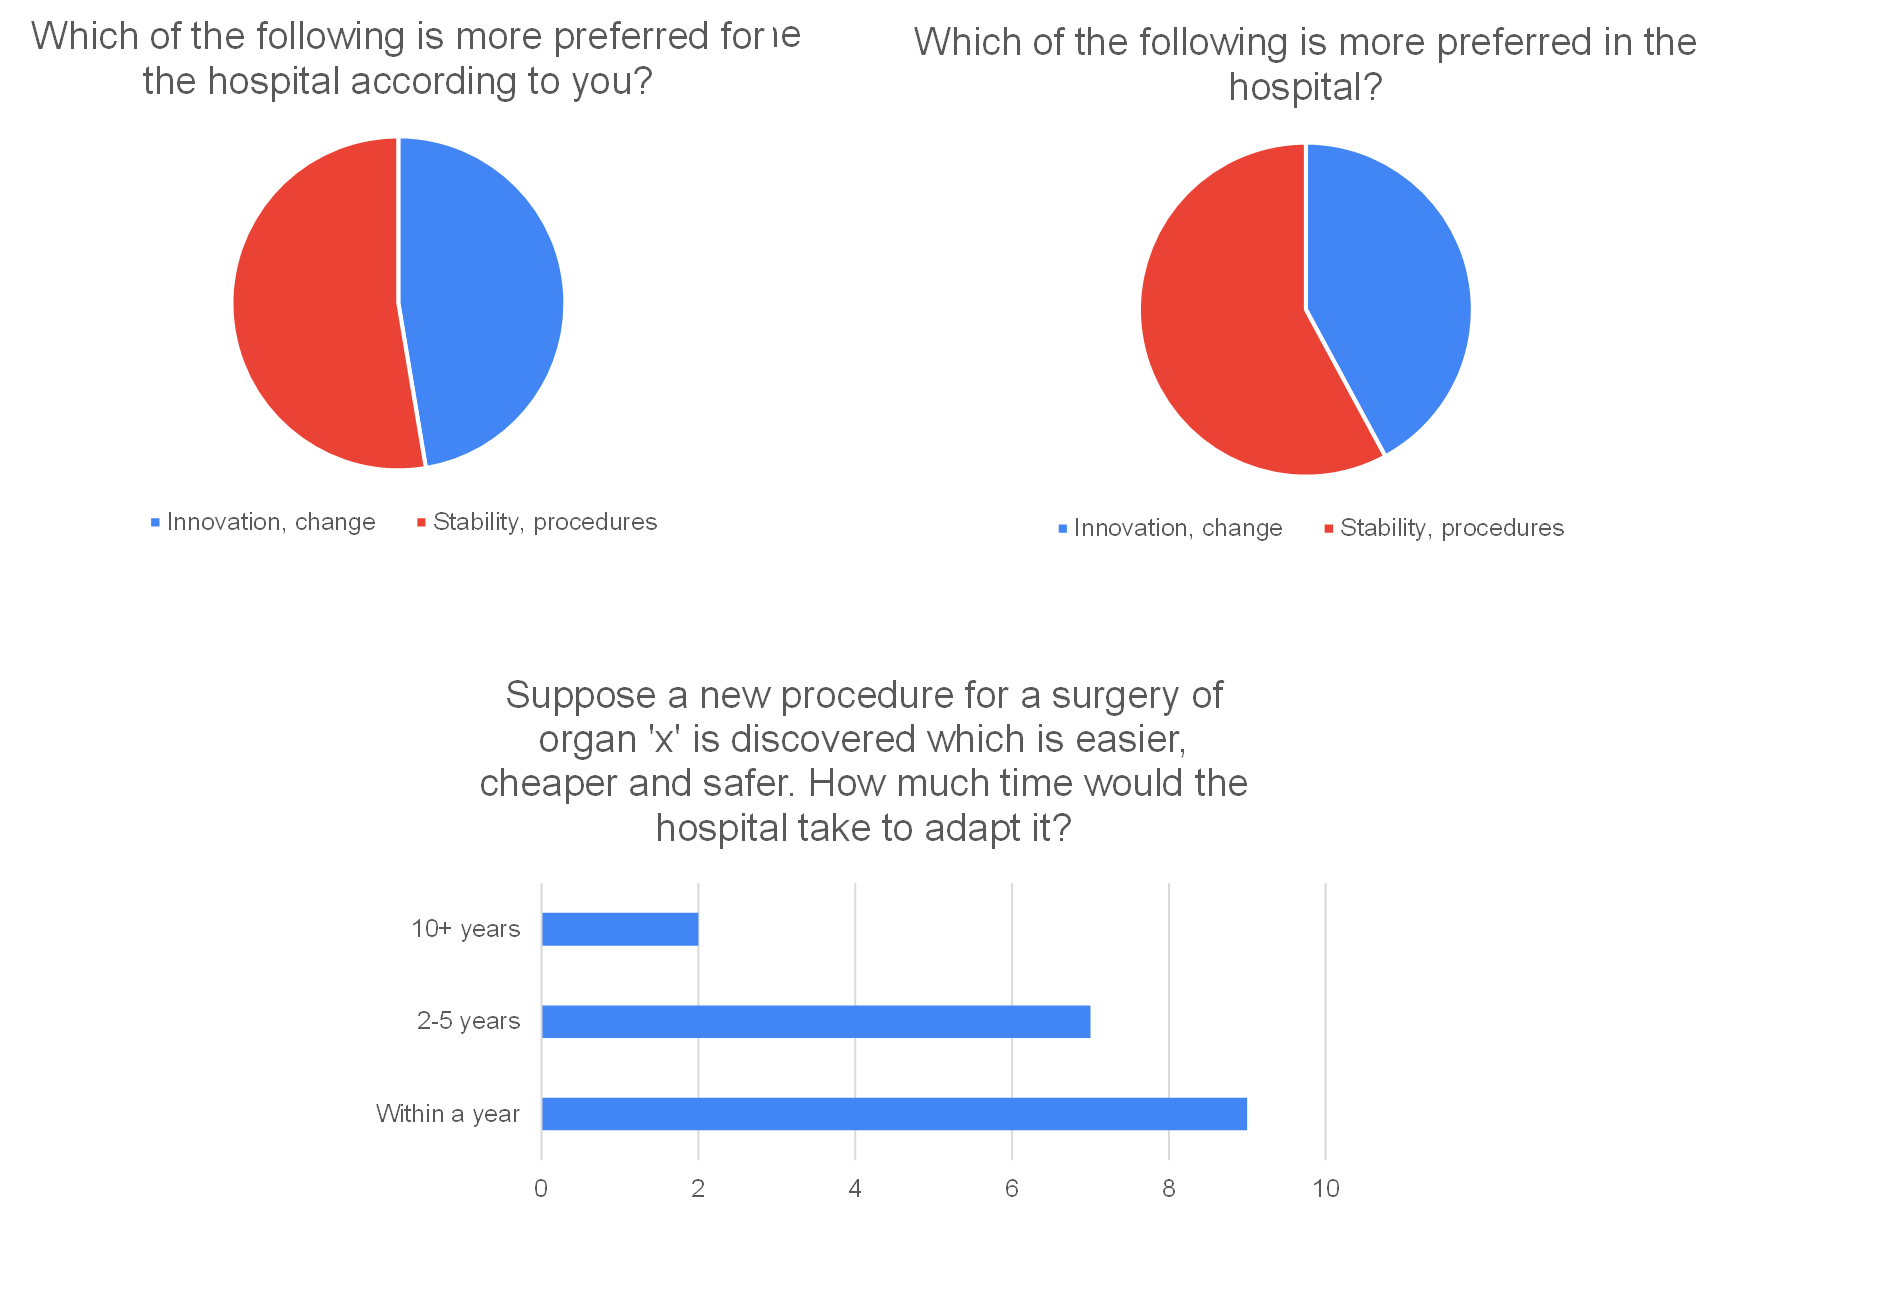
\includegraphics[width = 4in]{Time.png}
    \end{center}
    \caption{Responses of Questions Long-Term Orientation}
    \label{Time}
\end{figure}

\subsection{Individualistic or Collectivistic}

When it comes to responsibility for both success and failure, the majority (60\% and 50\%) voted it is shared between the team. The full result can be seen in Table \ref{responsible}. A point to note is that, amongst other options, when the matter of success came in, the responsibility of management was rated higher. This is a typical trait of a collectivistic organisation.

\begin{table}
    \begin{center}
        \begin{tabular}{|c|c|c|}
            \hline
            Responsible & Success & Failure \\
            \hline
            Head & 5 & 4\\
            Management & 5 & 1\\
            Whole team & 11 & 8\\
            \hline
        \end{tabular}
        \caption{Responses for Responsibility}
        \label{responsible}
    \end{center}
\end{table}

\subsection{Control vs Subjugation and communication}

In the last section of the form, questions related to control and communication were asked. When it comes to controlling, unlike the typical perspective, the employees felt that the power is not centralized to the head, and others also have some say in decision-making, along with the fact that the conflicts are generally solved internally.

We can also see the mode of communication sliding towards online communication, such as Whatsapp. Interestingly, the majority of the people who responded letters and emails as one of the mediums are officers at the hospital. Only 10\% of respondents said that communication is not transparent which is also very fitting that it is a government hospital.

\section{The Conclusion}

In conclusion, the analysis of the survey conducted at Civil Hospital has provided valuable insights into the reflection of national culture in the healthcare system of the country. The survey has revealed that the healthcare system is heavily influenced by cultural factors in a few aspects of culture, including hierarchical relationships, respect for authority, and collectivism. Meanwhile, it is not influenced strongly when it comes to certain attributes of national culture, such as uncertainty avoidance.

The result of Hofstede's study is true here, although some characteristics are not as strongly expressed as they seem to be in the ratings of India. According to the survey, the subjugation is not very high amongst the member, and hence the power distance would be low. The long-term orientation is still similar to what Hofstede finds. The extent of individualism also seems lower than what Hofstede found. However, one of the reasons can be the long-term posting of employees, which might create a close family-like structure amongst the employees. The dimension which is contrasting most is uncertainty avoidance. In general, the Indians tend to accept the uncertainty, but the hospital is also prepared for all basic uncertainties. This is probably the result of the healthcare system in which hospitals are obviously involved.

We can see this in making a play in the recent Covid-19 pandemic. Although it was an unpreceded event, India as a whole emerged strong from it while many advanced countries failed in such a strong response. Every member of the team worked for a long duration, and the whole team was awarded.

Still, we should keep in mind that the sample size used is only one hospital. Hence it should be generalized to all the hospitals in this vast country of $3.92\ km^2$ area.

\newpage
\begin{thebibliography}{99}

    \bibitem{ref:Hofstede's cultural dimensions theory}
    {Hofstede's cultural dimensions theory\\
    \url{https://en.wikipedia.org/wiki/Hofstede%27s_cultural_dimensions_theory#Dimensions_of_national_culturess}}


    \bibitem{ref:Hofstede's research on the national culture of India}
    {Hofstede's research on national culture of India\\
    \url{https://www.hofstede-insights.com/country-comparison/india/}}

    \bibitem{ref: IPCH}
    {Indian Public Health Standerds\\
    \url{https://nhm.gov.in/images/pdf/guidelines/iphs/iphs-revised-guidlines-2022/01-SDH_DH_IPHS_Guidelines-2022.pdf}}

    \bibitem{ref: Survey Form}
    {Survey Form\\
    \url{https://drive.google.com/file/d/1fBm0hNM2xrKJiMaiN55BHcJJa5gY-k8D/view?usp=share_link}}

    \bibitem{ref:Survey Results}
    {Survey of OB of Civil Hospital, Jalna (Responses)\\
    \url{https://docs.google.com/spreadsheets/d/13JBPbaedCzGmHHtawIFe-Poizsp84CtahEr07WUdKAw/edit?usp=sharing}}

\end{thebibliography}

\end{document}